\documentclass{article}
\usepackage{amsmath}
\usepackage{graphicx}  % For including images
\usepackage{hyperref}  % For hyperlinks
\usepackage{subcaption} % 用于子图
\setlength{\parindent}{2em} % 设置全局首行缩进为 2em

\begin{document}

\title{CS276 Homework 1: Light Field Rendering}
\author{Zhaoyu Qiu 2024192955\\ School of Biomedical Engineering \\ ShanghaiTech University }
\date{\today}
\maketitle

\section{Introduction}
\indent The purpose of this assignment is to perform refocusing based on light field data and to experiment with different aperture effects. The input for this assignment is a 16x16 image matrix, referencing classic projects such as Lytro camera data processing.

\section{Implement}

\subsection{Light Field Loading}
The 16x16 light field input used for the text is shown in Figure \ref{fig:light_field}.

\begin{figure}[ht]
    \centering
    \includegraphics[width=.7\textwidth]{./light_field_matrix.png}  % Replace with your image path
    \caption{16x16 Light Field Input}
    \label{fig:light_field}
\end{figure}

To create a light field, multiple images are captured from various viewpoints and organized into a 5D data structure, represented as:
\[
\text{Light Field}(u, v, x, y, c)
\]
where \( (u, v) \) represent the camera indices, \( (x, y) \) are the pixel coordinates, and \( c \) denotes the color channels. Each image is resized and stored in the array, ensuring uniform dimensions for accurate interpolation.

\subsection{Interpolation Resampling}
Interpolation is a crucial step in rendering the light field. Two primary interpolation methods are employed:

\subsubsection{Bilinear Interpolation}
For bilinear interpolation, the pixel value \( I(x, y) \) at an arbitrary position is calculated using:
\[
I(x, y) = w_a \cdot I_a + w_b \cdot I_b + w_c \cdot I_c + w_d \cdot I_d
\]
where \( w_a, w_b, w_c, w_d \) are the weights based on the neighboring pixel values.

\subsubsection{Trilinear Interpolation}
In a 3D light field, trilinear interpolation is utilized, which extends the bilinear approach into the depth dimension. The formula is given by:
\begin{align*}
    I(x, y, z) = & \, I_{000}(1-x)(1-y)(1-z) + I_{100}(x)(1-y)(1-z)\\
                  & \, + I_{010}(1-x)(y)(1-z) + I_{110}(x)(y)(1-z) \\
                  & \, + I_{001}(1-x)(1-y)(z) + I_{101}(x)(1-y)(z) \\
                  & \, + I_{011}(1-x)(y)(z) + I_{111}(x)(y)(z)
    \end{align*}
    

\subsection{Focal Plane Control}
Let the camera position be \( C = (x_c, y_c) \) and the focus distance be \( f \). The distance from a pixel point \( P = (x, y) \) to the camera position is calculated as:
\[
d = \sqrt{(x - x_c)^2 + (y - y_c)^2}
\]
The weight \( w \) for each camera view can be computed using the Gaussian function:
\[
w = \frac{1}{\sigma \sqrt{2\pi}} e^{-\frac{d^2}{2\sigma^2}}
\]
where \( \sigma \) is related to the aperture size, influencing the weight distribution.

\subsection{Aperture Control}
Let \( A \) be the aperture size, which affects the weight calculation. A larger aperture allows more camera views to contribute to the final image. The relationship can be described as:
\[
w \propto \frac{1}{A}
\]
This means that as the aperture increases, the weight distribution becomes flatter, impacting the clarity and detail of the final image.

\subsection{Z-Axis Control}
The focal length factor \( F \) simulates depth along the z-axis. The displacement in the x and y directions for each camera view can be calculated as:
\[
dx = (col - x_c) \cdot F \cdot \frac{width}{f}
\]
\[
dy = -(row - y_c) \cdot F \cdot \frac{height}{f}
\]
Here, \( (col, row) \) represents the position of the camera view, and \( (width, height) \) are the dimensions of the final image. The blur effect in the final image is controlled by the kernel size:
\[
\text{blur\_kernel\_size} = \max(1, \text{int}(F \cdot 2))
\]

\section{Experiments}
\subsection{GUI interface}
The user interface of this assignment consists of the components shown in the Figure \ref{fig:ui}, which includes 6 control sliders, 1 display page, and 1 confirm button.

As shown in Figure~\ref{fig:view_control}, the different perspectives are controlled and visualized.
\begin{figure}[htbp]
    \centering
    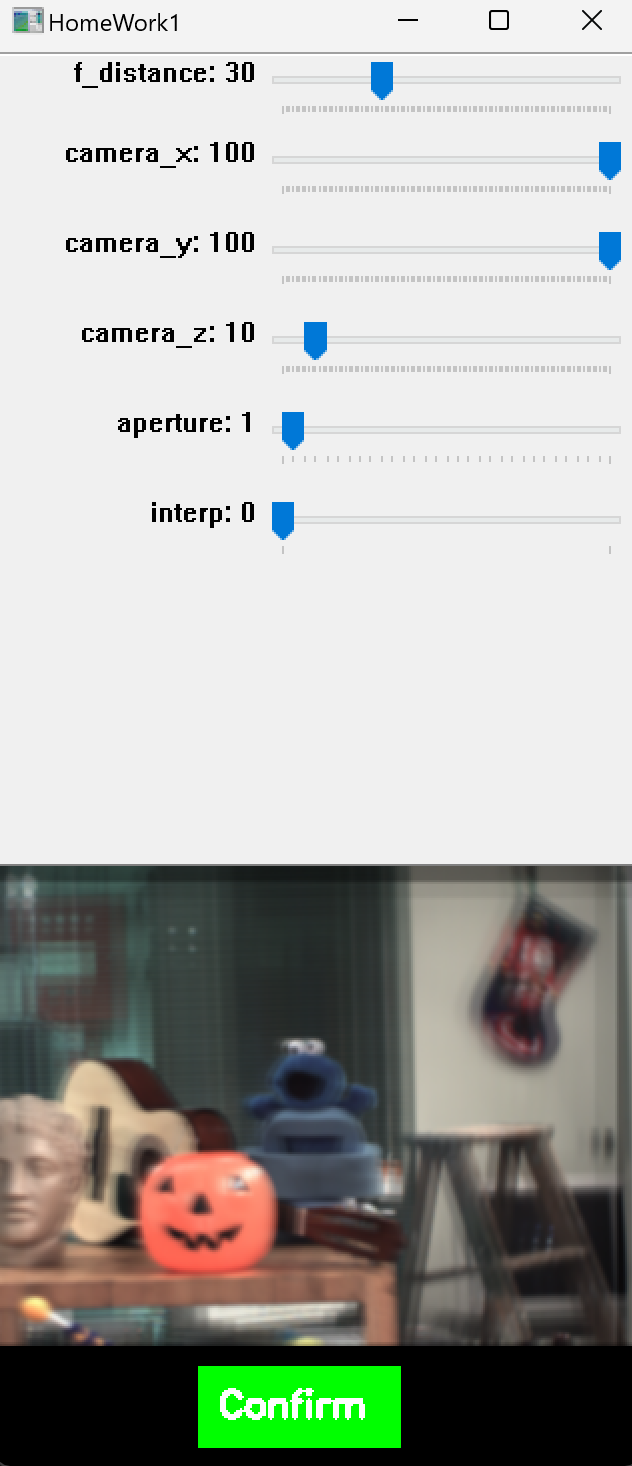
\includegraphics[width=0.35\textwidth]{GUI.png} % 替换为你的图片路径
    \caption{User interface overview}
    \label{fig:ui}
\end{figure}


\begin{figure}[htbp]
    \centering
    \begin{subfigure}[b]{0.23\textwidth} % Top-left subfigure
        \centering
        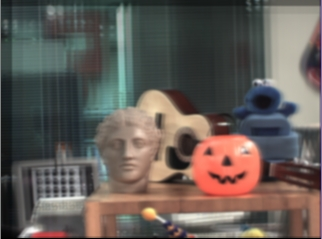
\includegraphics[width=\textwidth]{view1.png} % Replace with your image
        \caption{Top-left} % Subfigure caption
    \end{subfigure}
    \hfill
    \begin{subfigure}[b]{0.23\textwidth} % Top-right subfigure
        \centering
        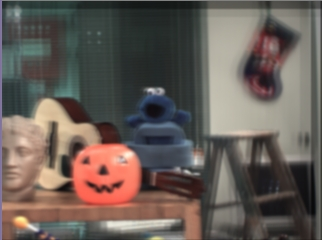
\includegraphics[width=\textwidth]{view2.png} % Replace with your image
        \caption{Top-right} % Subfigure caption
    \end{subfigure}
    \hfill
    \begin{subfigure}[b]{0.23\textwidth} % Bottom-left subfigure
        \centering
        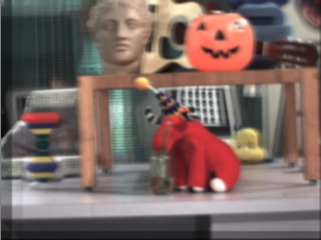
\includegraphics[width=\textwidth]{view3.png} % Replace with your image
        \caption{Bottom-left} % Subfigure caption
    \end{subfigure}
    \hfill
    \begin{subfigure}[b]{0.23\textwidth} % Bottom-right subfigure
        \centering
        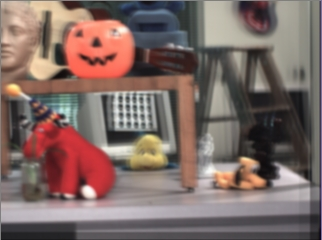
\includegraphics[width=\textwidth]{view4.png} % Replace with your image
        \caption{Bottom-right} % Subfigure caption
    \end{subfigure}
    
    \caption{Control of different perspectives: top-left, bottom-left, top-right, and bottom-right views.}
    \label{fig:view_control}
\end{figure}


\subsection{Interpolation Resampling}
The comparison of results between bilinear interpolation and trilinear interpolation is shown in Figure \ref{fig:interpolation}. In the relatively undersampled lower-left corner, the effect of multiple interpolations is superior.

\begin{figure}[htbp]
    \centering
    \begin{subfigure}{0.35\textwidth}
        \centering
        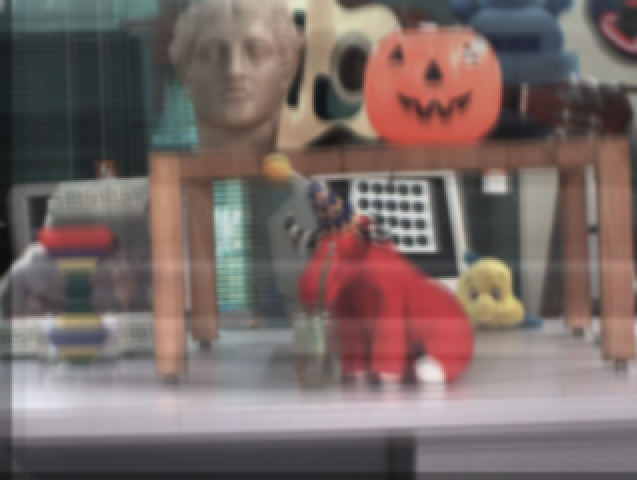
\includegraphics[width=\textwidth]{interp_2.png} % 替换为子图A的路径
        \caption{Bilinear interpolation}
        \label{fig:bilinear}
    \end{subfigure}%
    \begin{subfigure}{0.35\textwidth}
        \centering
        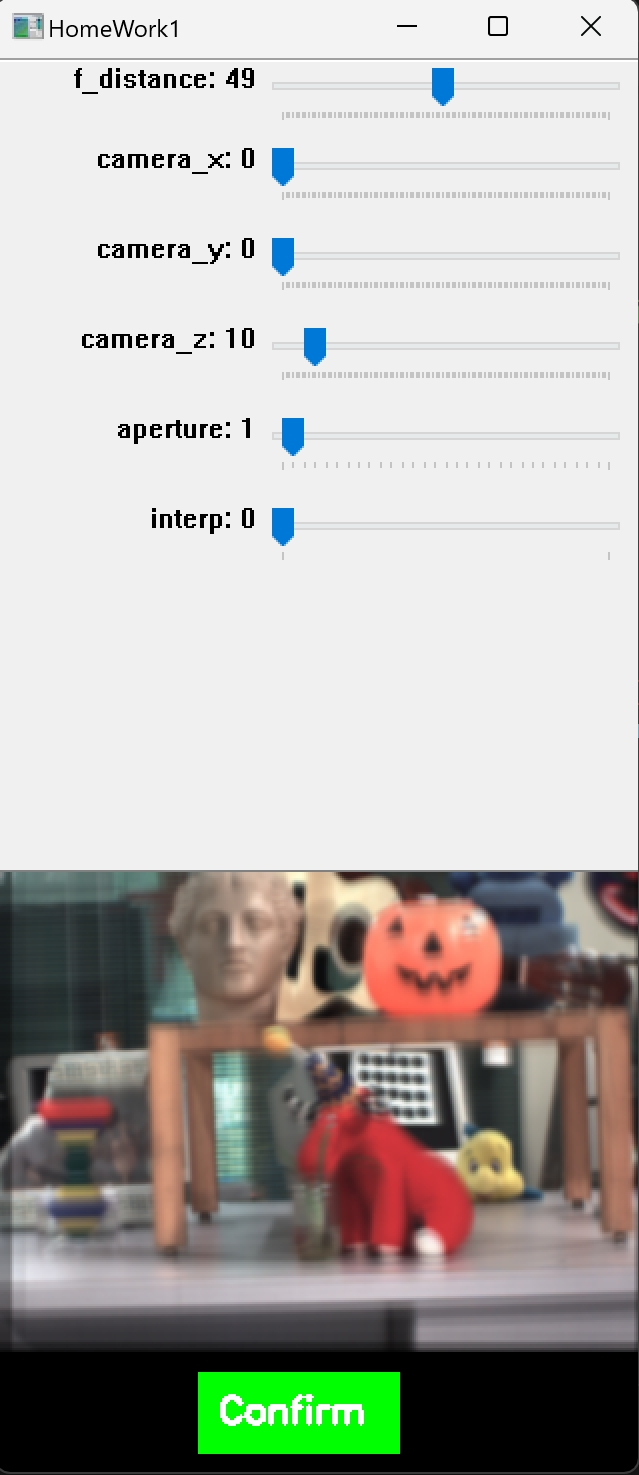
\includegraphics[width=\textwidth]{interp_4.png} % 替换为子图B的路径
        \caption{Trilinear interpolation}
        \label{fig:trilinear}
    \end{subfigure}
    \caption{Comparison of interpolation resampling}
    \label{fig:interpolation}
\end{figure}

\subsection{Focal Plane Control}

As shown in Figure~\ref{fig:f}, the effect of increasing focal length is illustrated.
\begin{figure}[htbp]
    \centering
    \begin{subfigure}[b]{0.32\textwidth} % First subfigure occupying 32% of the width
        \centering
        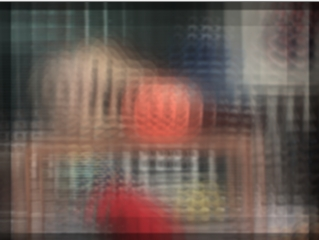
\includegraphics[width=\textwidth]{f1.png} % Replace with your image
        \caption{Focal length = 10} % Caption for the subfigure
    \end{subfigure}
    \hfill
    \begin{subfigure}[b]{0.32\textwidth} % Second subfigure
        \centering
        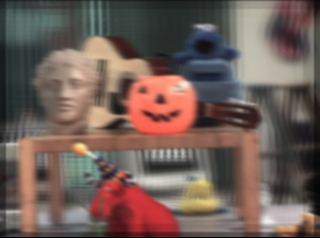
\includegraphics[width=\textwidth]{f12.png} % Replace with your image
        \caption{Focal length = 34} % Caption for the subfigure
    \end{subfigure}
    \hfill
    \begin{subfigure}[b]{0.32\textwidth} % Third subfigure
        \centering
        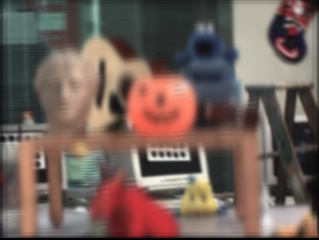
\includegraphics[width=\textwidth]{f3.png} % Replace with your image
        \caption{Focal length = 60} % Caption for the subfigure
    \end{subfigure}
    \caption{Effect of increasing focal length from small to large} % Overall figure caption
    \label{fig:f}
\end{figure}


\subsection{Aperture Control}
\begin{figure}[htbp]
    \begin{subfigure}[b]{0.24\textwidth} % Fourth subfigure
        \centering
        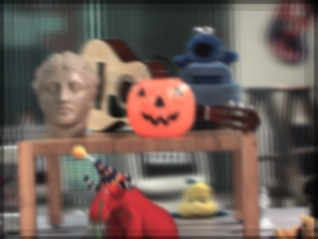
\includegraphics[width=\textwidth]{ap=0.png} % Replace with your image
        \caption{Aperture 1} % Subfigure caption
    \end{subfigure}
    \hfill
    \begin{subfigure}[b]{0.24\textwidth} % Third subfigure
        \centering
        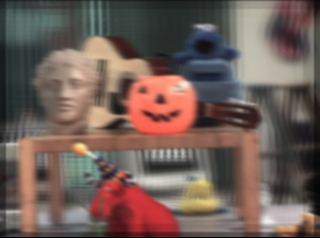
\includegraphics[width=\textwidth]{f12.png} % Replace with your image
        \caption{Aperture 2} % Subfigure caption
    \end{subfigure}
    \hfill
    \begin{subfigure}[b]{0.24\textwidth} % Second subfigure
        \centering
        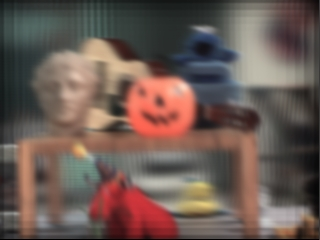
\includegraphics[width=\textwidth]{ap=2.png} % Replace with your image
        \caption{Aperture 3} % Subfigure caption
    \end{subfigure}
    \hfill
    \centering
    \begin{subfigure}[b]{0.24\textwidth} % First subfigure (25% of the width)
        \centering
        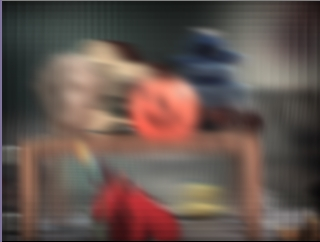
\includegraphics[width=\textwidth]{ap=4.png} % Replace with your image
        \caption{Aperture 4} % Subfigure caption
    \end{subfigure}

    \caption{Effect of different aperture sizes} % Overall figure caption
    \label{fig:aperture_example}
\end{figure}

As shown in Figure~\ref{fig:aperture_example}, the effect of different aperture sizes is illustrated.

\subsection{Z-Axis Control}
\begin{figure}[htbp]
    \centering
    \begin{subfigure}[b]{0.24\textwidth} % First subfigure
        \centering
        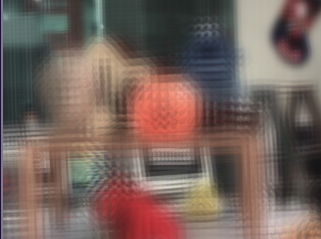
\includegraphics[width=\textwidth]{z=0.png} % Replace with your image
        \caption{Z = 0} % Subfigure caption
    \end{subfigure}
    \hfill
    \begin{subfigure}[b]{0.24\textwidth} % Second subfigure
        \centering
        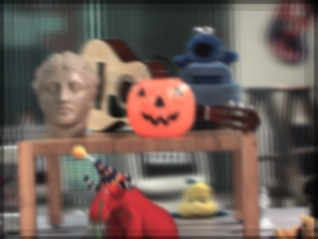
\includegraphics[width=\textwidth]{ap=0.png} % Replace with your image
        \caption{Z = 1} % Subfigure caption
    \end{subfigure}
    \hfill
    \begin{subfigure}[b]{0.24\textwidth} % Third subfigure
        \centering
        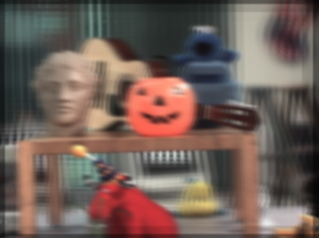
\includegraphics[width=\textwidth]{z=12.png} % Replace with your image
        \caption{Z = 12} % Subfigure caption
    \end{subfigure}
    \hfill
    \begin{subfigure}[b]{0.24\textwidth} % Fourth subfigure
        \centering
        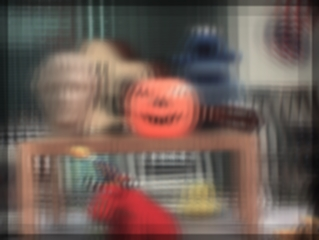
\includegraphics[width=\textwidth]{z=15.png} % Replace with your image
        \caption{Z = 15} % Subfigure caption
    \end{subfigure}
    
    \caption{Process of increasing Z-axis from small to large values}
    \label{fig:zaxis_example}
\end{figure}

As shown in Figure~\ref{fig:zaxis_example}, the Z-axis increases progressively in the illustrations.



\section{Conclusion}
This project implementation was inspired by two open-source projects: 
\href{https://github.com/chiped/LightFieldRenderer}{Open-source Project 1} and 
\href{https://github.com/TachikakaMin/Light_Field_Refocusing}{Open-source Project 2}.

The final implementation achieved three main tasks: interpolation, view control, and focus control. Since this is my first time handling light field data, I think the aperture control and Z-axis control may not be entirely correct. I look forward to reviewing and learning from other students.


\end{document}
